\documentclass[12pt,a4paper]{article}

% -------------------------------------------------
% PACKAGES
% -------------------------------------------------
\usepackage[a4paper,margin=2.5cm]{geometry}
\usepackage[T1]{fontenc}
\usepackage[utf8]{inputenc}
\usepackage{lmodern}
\usepackage{setspace}
\usepackage{hyperref}
\usepackage{xcolor}
\usepackage{graphicx}
\usepackage{float}
\usepackage{booktabs}
\usepackage{longtable}
\usepackage{array}
\usepackage{enumitem}
\usepackage{listings}
\usepackage{caption}
\usepackage{float}
\usepackage{booktabs}
\usepackage{tabularx}
\usepackage{array}
\usepackage{svg}


% -------------------------------------------------
% HYPERREF SETUP
% -------------------------------------------------
\hypersetup{
	colorlinks=true,
	linkcolor=black,
	urlcolor=blue,
	citecolor=black,
	pdftitle={Raw Formula 1 Data Re-engineering for a Reconciled PostgreSQL Database},
	pdfauthor={Author Name},
	pdfsubject={Data re-engineering},
	pdfkeywords={FastF1, Ergast, PostgreSQL, reconciled database, Formula 1}
}

% -------------------------------------------------
% SPACING
% -------------------------------------------------
\onehalfspacing

% -------------------------------------------------
% LISTINGS
% -------------------------------------------------
\definecolor{codebg}{RGB}{248,248,248}
\definecolor{codeframe}{RGB}{220,220,220}
\definecolor{codecomment}{RGB}{90,90,90}
\definecolor{codekeyword}{RGB}{0,0,120}
\definecolor{codestring}{RGB}{120,40,0}

\lstdefinestyle{pythonstyle}{
	language=Python,
	backgroundcolor=\color{codebg},
	frame=single,
	rulecolor=\color{codeframe},
	basicstyle=\ttfamily\small,
	keywordstyle=\color{codekeyword}\bfseries,
	commentstyle=\color{codecomment}\itshape,
	stringstyle=\color{codestring},
	breaklines=true,
	showstringspaces=false,
	tabsize=4
}

\lstdefinestyle{sqlstyle}{
	language=SQL,
	backgroundcolor=\color{codebg},
	frame=single,
	rulecolor=\color{codeframe},
	basicstyle=\ttfamily\small,
	keywordstyle=\color{codekeyword}\bfseries,
	commentstyle=\color{codecomment}\itshape,
	stringstyle=\color{codestring},
	breaklines=true,
	showstringspaces=false,
	tabsize=4
}

% -------------------------------------------------
% PLACEHOLDER COMMANDS
% -------------------------------------------------
\newcommand{\placeholder}[1]{%
	\par\noindent\textcolor{gray}{\textit{#1}}\par
}

\newcommand{\important}[1]{%
	\par\noindent\textbf{#1}\par
}

% -------------------------------------------------
% TITLE
% -------------------------------------------------
\title{\textbf{Raw Formula 1 Data Re-engineering\\for a Reconciled PostgreSQL Database}}
\author{Giuseppe Rudi}
\date{\today}

% -------------------------------------------------
% DOCUMENT
% -------------------------------------------------
\begin{document}
	
	\maketitle
	\tableofcontents
	\newpage
	
	% =================================================
	\section{Introduction}
	% =================================================
	
	This document focuses only on the re-engineering of raw Formula 1 data extracted from FastF1 and Ergast, with the purpose of obtaining a relational structure suitable for a reconciled PostgreSQL database.
	
	This report does not discuss data quality assessment, error correction, or cleaning metrics. Those topics will be presented in a separate document after the data import and schema consolidation phases are completed.
	

	
	The main objective is to transform raw API-oriented data into database-friendly relations with explicit keys, clear cardinalities, stable identifiers, and meaningful links between tables.
	
	% =================================================
	\section{Data Sources}
	% =================================================
	
	The data sources used in this project can be divided into two main categories:
	API-based sources and externally constructed domain tables.
	
	\subsection{FastF1 as Main Source}
	FastF1 is the main source used in the project.
	It provides most of the race-related data needed to build the reconciled database, including event-level information, session-level information, lap data, timing-related attributes, weather data, track status data, and other structures related to Formula 1 weekends.
	
	\subsection{Ergast as Supporting Source}
	Ergast is used as a supporting source for master data.
	In particular, it provides historical information about drivers and constructors, which is used to build the \texttt{Driver} and \texttt{Team} tables.
	Although Ergast is a distinct source, it is accessed in this project through the FastF1 interface, which provides a bridge to the Ergast/Jolpica API.
	
	\subsection{Domain Tables Built from External Knowledge}
	Some tables of the reconciled database are not directly extracted from FastF1 or Ergast.
	Instead, they are introduced through domain knowledge and external descriptive sources.
	This is the case, for example, of the \texttt{Season} and \texttt{Circuit} tables.
	These relations are created manually in order to include information that is not directly available in the API extraction workflow, but is still necessary to support the analytical goals of the project.
	
	
	

	% =================================================
	\section{Re-engineering of Individual Raw Structures}
	% =================================================
	
	
	\subsection{Naming Standardization: From API Naming to Snake Case}
	
	
	The structures returned by the FastF1 API use names that are suitable for programmatic objects, but are less convenient for relational database design.
	In particular, many attributes are written without separators and with an uppercase initial letter for each word, such as \textit{SeasonYear}, \textit{SessionType}.
	This naming style is known as  \textit{UpperCamelCase}.
	
	For database design, a more common and professional convention is \textit{snake\_case}, where words are written in lowercase and separated by underscores.
	
	For this reason, during the re-engineering phase, table names and attribute names were normalized from the original API-oriented style to snake\_case.

	
	Therefore, the adoption of snake\_case was not only a cosmetic modification, but a deliberate normalization step aimed at producing a cleaner and more database-oriented reconciled schema.
	
	\subsection{Season}
	
	Before re-engineering the raw event schedule, a \texttt{Season} table was introduced in order to explicitly represent the Formula 1 season as an independent entity in the reconciled database.
	Unlike the other tables of the reconciled schema, this relation is not directly extracted from FastF1 or Ergast.
	Instead, it is created from the analytical scope defined for the project and enriched with additional domain information collected from official external sources.
	

	
	\begin{table}[H]
		\centering
		\caption{Attributes of the current \texttt{season} table}
		\renewcommand{\arraystretch}{1.15}
		\begin{tabularx}{0.9\textwidth}{>{\raggedright\arraybackslash}X >{\raggedright\arraybackslash}X >{\raggedright\arraybackslash}X}
			\toprule
			\textbf{Attribute} & \textbf{Attribute} & \textbf{Attribute} \\
			\midrule
			\texttt{season\_year} & \texttt{season\_end\_date} & \texttt{champion\_driver} \\
			\texttt{season\_start\_date} & \texttt{number\_of\_events} & \texttt{champion\_team} \\
			\bottomrule
		\end{tabularx}
	\end{table}
	
	From a relational point of view, \texttt{SeasonYear} is the primary key of the \texttt{Season} table.
	This design choice provides a clear parent relation for the event-level and session-level parts of the reconciled database.
	In particular, \texttt{SeasonYear} is later propagated to the \texttt{Grand Prix} table, where it acts as a foreign key and connects each event weekend to the corresponding Formula 1 season.
	

	Only the choice of the seasons to be analyzed comes from the project scope, while the additional championship-level attributes are introduced through domain knowledge and official external sources.
	
	For documentation purposes, the information used to populate this table was obtained from the official Formula 1 calendar and standings pages:
	\begin{itemize}
		\item 2021 calendar: \url{https://www.formula1.com/en/racing/2021}
		\item 2022 calendar: \url{https://www.formula1.com/en/racing/2022}
		\item 2021 Drivers' Standings: \url{https://www.formula1.com/en/results/2021/drivers}
		\item 2022 Drivers' Standings: \url{https://www.formula1.com/en/results/2022/drivers}
		\item 2021 Teams' Standings: \url{https://www.formula1.com/en/results/2021/team}
		\item 2022 Teams' Standings: \url{https://www.formula1.com/en/results/2022/team}
	\end{itemize}
	
	
	\subsection{Circuit}
	
	The \texttt{circuit} table was not derived from FastF1, Ergast, or any other API directly used for the extraction of session-level and lap-level data.
	Instead, it was introduced as an additional domain table in the reconciled database in order to support one of the analytical goals of the project, namely the interpretation of team and driver performance with respect to circuit characteristics and sector typology.
	
	In particular, this table was designed to provide a structured classification of each circuit and of its three sectors.
	This classification is useful to study whether some cars or teams perform better in specific technical contexts, such as power-sensitive sectors, high-speed corners, technical sections, or street-track environments.


	\begin{table}[H]
		\centering
		\caption{Attributes of the \texttt{circuit} table (snake\_case)}
		\renewcommand{\arraystretch}{1.15}
		\begin{tabularx}{\textwidth}{>{\raggedright\arraybackslash}X >{\raggedright\arraybackslash}X >{\raggedright\arraybackslash}X}
			\toprule
			\textbf{Attribute} & \textbf{Attribute} & \textbf{Attribute} \\
			\midrule
			\texttt{circuit\_id} & \texttt{location} & \texttt{sector1\_category} \\
			\texttt{circuit\_name} & \texttt{seasons\_present} & \texttt{sector2\_category} \\
			\texttt{country} & \texttt{global\_circuit\_category} & \texttt{sector3\_category} \\
			\bottomrule
		\end{tabularx}
	\end{table}
	
	From a conceptual point of view, the relationship between \texttt{circuit} and \texttt{grand Prix} is one-to-many.
	A single circuit may host multiple race weekends across one or more seasons, while each race weekend is associated with exactly one circuit.
	For this reason, in the logical schema the attribute \texttt{circuit\_id} is used as the primary key of the \texttt{circuit} table and as a foreign key in the \texttt{grand Prix} table.
	
	A relevant aspect of this re-engineering step is that the \texttt{circuit} table cannot be obtained automatically from the raw FastF1 schedule alone.
	The raw \texttt{grand Prix} data do not directly expose a circuit identifier compatible with the target schema.
	Therefore, the integration requires an additional matching step between the reconciled \texttt{grand Prix} table and the manually created \texttt{circuit} table.
	
	The most reliable matching strategy is based on the pair \texttt{country} and \texttt{location}.
	Using only \texttt{country} would not be sufficient, because different race weekends may take place in the same country.
	By contrast, the combination of \texttt{country} and \texttt{location} provides a much more precise criterion to associate each grand prix with the correct circuit.
	For this reason, the integration can be carried out through a semi-automatic script that matches the two tables on these attributes, followed by a manual validation step.
	
	Operationally, the re-engineering process consists of two parts.
	First, the \texttt{circuit} table is created manually from domain knowledge and external descriptive sources.
	Second, the reconciled \texttt{Grand Prix} table is enriched with the foreign key \texttt{CircuitId} by matching each grand prix with the corresponding circuit through \texttt{Country} and \texttt{Location}.
	
	\begin{table}[H]
		\centering
		\caption{Summary of the re-engineering operations}
		\renewcommand{\arraystretch}{1.2}
		\begin{tabularx}{\textwidth}{>{\raggedright\arraybackslash}p{4.2cm} >{\raggedright\arraybackslash}p{3.0cm} >{\raggedright\arraybackslash}X}
			\toprule
			\textbf{Operation} & \textbf{Applied to} & \textbf{Purpose} \\
			\midrule
			Introduction of the \texttt{Circuit} relation & Reconciled database design & To represent circuit-level technical knowledge not available in the raw API sources \\
			\addlinespace
			Definition of circuit and sector categories & \texttt{Circuit} table & To support the interpretation of performance differences across different types of tracks and sectors \\
			\addlinespace
			Definition of \texttt{CircuitId} as primary key & \texttt{Circuit} table & To uniquely identify each circuit in the reconciled schema \\
			\addlinespace
			Addition of \texttt{CircuitId} as foreign key & \texttt{Grand Prix} table & To connect each race weekend to the circuit where it takes place \\
			\addlinespace
			Semi-automatic matching on \texttt{Country} and \texttt{Location} & \texttt{Grand Prix} and \texttt{Circuit} tables & To integrate circuit information into event-level data with a reliable matching rule \\
			\addlinespace
			Manual validation of matched records & Integration step & To confirm the correctness of the circuit assignment and resolve possible naming inconsistencies \\
			\bottomrule
		\end{tabularx}
	\end{table}
	
	
	\subsection{Grand Prix and Session}
	
	The raw structure returned by \texttt{FastF1.get\_event\_schedule(year)} was used as the starting point for the design of the event-related part of the reconciled database.
	This structure contains one row for each Formula 1 Grand Prix in a given season, but it mixes in the same object both general event information and session-related information.
	For this reason, it was not stored directly in the reconciled database.
	Instead, it was re-engineered into two separate relations: \texttt{grand Prix} and \texttt{session}.
	
	\begin{table}[H]
		\centering
		\caption{Attributes of the raw FastF1 schedule}
		\renewcommand{\arraystretch}{1.15}
		\begin{tabularx}{\textwidth}{>{\raggedright\arraybackslash}X >{\raggedright\arraybackslash}X >{\raggedright\arraybackslash}X}
			\toprule
			\textbf{Attribute} & \textbf{Attribute} & \textbf{Attribute} \\
			\midrule
			\texttt{RoundNumber} & \texttt{Country} & \texttt{Location} \\
			\texttt{OfficialEventName} & \texttt{EventDate} & \texttt{EventName} \\
			\texttt{EventFormat} & \texttt{F1ApiSupport} & \\
			\texttt{Session1} & \texttt{Session1Date} & \texttt{Session1DateUtc} \\
			\texttt{Session2} & \texttt{Session2Date} & \texttt{Session2DateUtc} \\
			\texttt{Session3} & \texttt{Session3Date} & \texttt{Session3DateUtc} \\
			\texttt{Session4} & \texttt{Session4Date} & \texttt{Session4DateUtc} \\
			\texttt{Session5} & \texttt{Session5Date} & \texttt{Session5DateUtc} \\
			\bottomrule
		\end{tabularx}
	\end{table}
	
	A first re-engineering step was the explicit addition of the attribute \texttt{season\_year}, which is necessary to connect the Grand Prix to the corresponding Formula 1 season.
	This attribute becomes the primary key of the \texttt{season} table and is also propagated to the derived relations.
	
	The main structural transformation was the split of the raw schedule into two different tables.
	The \texttt{grand\_prix} table stores only the attributes that describe the Grand Prix weekend at a general level, while the \texttt{session} table stores only the session-level information needed for the project.
	This second relation is introduced as a result of the re-engineering process, because in the raw FastF1 schedule the session information is embedded in the event structure and is not modeled as a separate relational table.
	
	
	A further filtering step was the exclusion of testing events from the reconciled schema.
	Although these events are returned by the raw FastF1 schedule, they are not part of the championship race calendar and are not consistent with the round-based structure adopted in the database design.

	\begin{table}[H]
		\centering
		\caption{Attributes of the final \texttt{grand\_prix} table}
		\renewcommand{\arraystretch}{1.15}
		\begin{tabularx}{\textwidth}{>{\raggedright\arraybackslash}X >{\raggedright\arraybackslash}X >{\raggedright\arraybackslash}X}
			\toprule
			\textbf{Attribute} & \textbf{Attribute} & \textbf{Attribute} \\
			\midrule
			\texttt{season\_year}         & \texttt{grand\_prix\_id}       & \texttt{event\_date} \\
			\texttt{round\_number}        & \texttt{country}               & \texttt{event\_format} \\
			\texttt{event\_name}          & \texttt{location}              & \texttt{f1\_api\_support} \\
			\texttt{circuit\_id}          & \texttt{official\_event\_name}  &                         \\
			\bottomrule
		\end{tabularx}
	\end{table}
	
	From a relational point of view, the \texttt{grand\_prix} table is identified by surrogate primary key  \texttt{grand\_prix\_id}.
	Furthermore \texttt{season\_year} is a foreign key referencing the \texttt{season} table, since each grand prix belongs to exactly one Formula 1 season.
	In addition, the attribute \texttt{circuit\_id} was introduced in the \texttt{grand\_prix} table as a foreign key toward the manually constructed \texttt{circuit} relation.
	
	\begin{table}[H]
		\centering
		\caption{Attributes of the final \texttt{session} table}
		\renewcommand{\arraystretch}{1.15}
		\begin{tabularx}{0.9\textwidth}{>{\raggedright\arraybackslash}X >{\raggedright\arraybackslash}X >{\raggedright\arraybackslash}X}
			\toprule
			\textbf{Attribute} & \textbf{Attribute} & \textbf{Attribute} \\
			\midrule
			\texttt{session\_id}  & \texttt{session\_type} & \texttt{session\_date} \\
			\texttt{grand\_prix\_id} & \texttt{session\_name} &  \\
			\bottomrule
		\end{tabularx}
	\end{table}
		
	The \texttt{session} table is identified by the surrogate primary key \texttt{session\_id}.
	Moreover, the \texttt{grand\_prix\_id} is also a foreign key referencing the \texttt{grand\_prix} table.
	
	
	During the re-engineering phase, only the session types relevant to the analytical goal of the project were retained.
	In particular, the reconciled \texttt{session} table includes only Qualifying and Race sessions.
	
	This choice was made because the project focuses on performance analysis in comparable competitive contexts.
	Free practice sessions were not included, since they are mainly used by teams for testing, setup work, tyre evaluation, and race preparation.
	For this reason, their data are less suitable for a clean comparison of driver and team performance.
	
	Excluding free practice sessions during re-engineering avoids carrying unnecessary data into the reconciled database and, later, into the Data Warehouse.
	This makes the schema more coherent with the business questions and reduces the amount of data that would otherwise have to be filtered out only at the analytical stage.
	
	\begin{table}[H]
		\centering
		\caption{Summary of the re-engineering operations applied to the raw schedule}
		\renewcommand{\arraystretch}{1.2}
		\begin{tabularx}{\textwidth}{>{\raggedright\arraybackslash}p{3.6cm} >{\raggedright\arraybackslash}p{3.2cm} >{\raggedright\arraybackslash}X}
			\toprule
			\textbf{Operation} & \textbf{Applied to} & \textbf{Purpose} \\
			\midrule

			Exclusion of testing events & Raw schedule & To remove non-championship events that are not compatible with the round-based structure of the reconciled database  \\
			\addlinespace
			Addition of \texttt{SeasonYear} & Grand Prix  Table & To explicitly connect each grand prix to the corresponding Formula 1 season \\
			\addlinespace
			Splitting of the raw schedule into \texttt{Grand Prix} and \texttt{Session} & Raw schedule & To separate event-level information from session-level information and assign to each relation only its correct attributes \\
			\addlinespace
			Restriction to Qualifying and Race & \texttt{Session} table & To keep only the sessions relevant for the analytical scope of the project \\
			\addlinespace
			Create surrogate primary keys & \texttt{Grand Prix} and \texttt{Session} & To uniquely identify rows at the correct granularity \\
			\addlinespace
			Foreign key relationship & \texttt{Session} toward \texttt{Grand Prix} & To represent that each session belongs to one specific grand prix \\
			\addlinespace
			Addition of \texttt{CircuitId} & \texttt{Grand Prix} table & To connect each grand prix weekend to the corresponding circuit \\
			\bottomrule
		\end{tabularx}
	\end{table}
	
	This redesign makes the schema more coherent with the real structure of a Formula 1 season:
	a season contains multiple grand prixs, and each grand prix contains multiple sessions.
	At the same time, it produces a cleaner and more database-friendly structure, because each relation stores information at only one semantic level.
	
	
	\subsection{Driver and Team}
	
	The \texttt{driver} and \texttt{team} tables were not extracted from the raw FastF1 event schedule.
	Instead, they were obtained from the Ergast/Jolpica source through the FastF1 \texttt{Ergast} interface.

	
	\begin{table}[H]
		\centering
		\caption{Attributes of the final \texttt{driver} table}
		\renewcommand{\arraystretch}{1.15}
		\begin{tabularx}{0.95\textwidth}{>{\raggedright\arraybackslash}X >{\raggedright\arraybackslash}X >{\raggedright\arraybackslash}X}
			\toprule
			\textbf{Attribute} & \textbf{Attribute} & \textbf{Attribute} \\
			\midrule
			\texttt{driver\_id}         & \texttt{abbreviation}    & \texttt{date\_of\_birth} \\
			\texttt{permanent\_number}  & \texttt{first\_name}     & \texttt{nationality} \\
			\texttt{last\_name}         & \texttt{driver\_url}     & \\
			\bottomrule
		\end{tabularx}
	\end{table}
	
	\begin{table}[H]
		\centering
		\caption{Attributes of the final \texttt{team} table}
		\renewcommand{\arraystretch}{1.15}
		\begin{tabularx}{0.75\textwidth}{>{\raggedright\arraybackslash}X >{\raggedright\arraybackslash}X}
			\toprule
			\textbf{Attribute} & \textbf{Attribute} \\
			\midrule
			\texttt{team\_id}      & \texttt{nationality} \\
			\texttt{team\_name}    & \texttt{team\_url} \\
			\bottomrule
		\end{tabularx}
	\end{table}
		
	The raw \texttt{driver} and \texttt{team} data structures are not reported separately, since their attribute sets were already very close to the final reconciled ones. Therefore, no substantial attribute-level re-engineering was required, apart from naming standardization.
	

	
	In the initial design, the relationships between \texttt{season} and \texttt{driver}, and between
	\texttt{season} and \texttt{team}, were represented through two associative tables:
	\texttt{season\_driver} and \texttt{season\_team}.
	
	However, this design was later revised in order to avoid redundant relationships in the
	reconciled schema. Drivers and teams are not connected directly to seasons anymore.
	Instead, their participation in a season can be derived through the dynamic tables of the
	domain, namely \texttt{result} and \texttt{lap}.
	
	From a conceptual point of view, a driver can perform many laps, while each lap is
	performed by exactly one driver. The same reasoning applies to teams: a team can be
	associated with many laps, while each lap is associated with exactly one team.
	
	Therefore, the relationship between \texttt{driver} and \texttt{lap} is one-to-many, and the
	relationship between \texttt{team} and \texttt{lap} is also one-to-many.
	
	The \texttt{result} table represents the result of one driver, belonging to one team, in one
	specific session. For this reason, each result row is associated with exactly one driver and
	exactly one team. At the same time, the same driver or team can appear in many result
	rows across different sessions.
	
	For this reason, the primary keys \texttt{driver\_id} and \texttt{team\_id} are stored as foreign
	keys in both \texttt{lap} and \texttt{result}. This allows the schema to connect performance
	data directly to the driver and team involved in each lap or session result.
	

	
	A further important point concerns identifier consistency.
	Within FastF1 session results, the attributes \texttt{driver\_id} and \texttt{team\_id} are explicitly documented as the identifiers used by Ergast.

	
	\paragraph{Note on the Driver-Team relationship}
	
	In the current reconciled schema, the relationship between \texttt{driver} and
	\texttt{team} is not modeled as a direct association.
	
	This is a deliberate design choice. A direct relationship between a driver and a team
	would not be sufficient to correctly represent the Formula 1 domain, because the
	association between a driver and a team is time-dependent. A driver may belong to one
	team in a season and to a different team in another season. Therefore, the association
	would require at least the season context.
	
	In the current project, this relationship is not materialized as a separate table because
	the main analytical focus is not the reconstruction of driver careers or official team
	line-ups. The focus is instead on the performance of teams and cars across sessions,
	Grand Prix events, circuits, tyres, and seasons.
	
	The information about which driver was associated with which team in a given session
	can still be derived from the dynamic tables of the schema, in particular from
	\texttt{lap} and \texttt{result}. Both relations contain the identifiers \texttt{driver\_id}
	and \texttt{team\_id}, and they are connected to \texttt{session}, \texttt{grand\_prix},
	and \texttt{season}. Therefore, the driver-team-season association can be reconstructed
	through queries when needed.
	
	A possible future extension of the schema could introduce an explicit associative table,
	such as:
	
	\begin{quote}
		\texttt{season\_driver\_team(season\_year, driver\_id, team\_id)}
	\end{quote}
	

	Such an extension would be useful if the project were focused on driver-team
	affiliations, driver transfers, or career evolution. However, for the current analytical
	scope, deriving this information from \texttt{lap} and \texttt{result} is sufficient and
	avoids adding redundant relationships to the reconciled schema.
	
	\subsection{Result}
	
	The \texttt{result} table was derived from the \texttt{session.results} object returned by FastF1 after loading a specific session.
	This raw structure contains both result-level information and several descriptive attributes related to drivers and teams.

	\begin{table}[H]
		\centering
		\caption{Attributes of the raw FastF1 \texttt{session.results} object}
		\renewcommand{\arraystretch}{1.15}
		\begin{tabularx}{\textwidth}{>{\raggedright\arraybackslash}X >{\raggedright\arraybackslash}X >{\raggedright\arraybackslash}X}
			\toprule
			\textbf{Attribute} & \textbf{Attribute} & \textbf{Attribute} \\
			\midrule
			\texttt{DriverNumber} & \texttt{TeamName} & \texttt{CountryCode} \\
			\texttt{BroadcastName} & \texttt{TeamColor} & \texttt{Position} \\
			\texttt{Abbreviation} & \texttt{TeamId} & \texttt{ClassifiedPosition} \\
			\texttt{DriverId} & \texttt{FirstName} & \texttt{GridPosition} \\
			\texttt{FullName} & \texttt{LastName} & \texttt{Q1} \\
			\texttt{HeadshotUrl} & \texttt{Q2} & \texttt{Q3} \\
			\texttt{Time} & \texttt{Status} & \texttt{Points} \\
			\multicolumn{3}{l}{\texttt{Laps}} \\
			\bottomrule
		\end{tabularx}
	\end{table}
	

	Attributes related to driver identity and team description  are not necessary in the final reconciled table because they can be recovered through relational joins based on \texttt{driver\_id} and \texttt{team\_id}.
	
	A further re-engineering step was the addition of the structural attribute \texttt{session\_id}
	necessary to connect each result to the corresponding session.

	
	Another important re-engineering choice concerns time-related columns.
	In the raw FastF1 results, attributes such as \texttt{Q1}, \texttt{Q2}, \texttt{Q3}, and \texttt{Time} are represented as timedelta values.
	For database clarity and easier numerical comparison, these columns were converted into integer milliseconds and renamed with the suffix \texttt{\_ms}.
	In the final reconciled schema, only the converted millisecond-based representation is stored, in order to avoid redundancy between two equivalent formats of the same information.
	
	\begin{table}[H]
		\centering
		\caption{Attributes of the final \texttt{result} table}
		\renewcommand{\arraystretch}{1.15}
		\begin{tabularx}{0.95\textwidth}{>{\raggedright\arraybackslash}X >{\raggedright\arraybackslash}X >{\raggedright\arraybackslash}X}
			\toprule
			\textbf{Attribute} & \textbf{Attribute} & \textbf{Attribute} \\
			\midrule
			\texttt{result\_id}            & \texttt{position}              & \texttt{q3\_ms} \\
			\texttt{session\_id}         & \texttt{classified\_position}  & \texttt{time\_ms} \\
			\texttt{laps}                & \texttt{grid\_position}        & \texttt{status} \\
			\texttt{driver\_id}            & \texttt{q1\_ms}                & \texttt{points} \\
			\texttt{team\_id}              & \texttt{q2\_ms}                &  \\
			\bottomrule
		\end{tabularx}
	\end{table}

	The attribute \texttt{grid\_position} is stored as a nullable integer. It is a
	race-context attribute: values greater than or equal to zero are admitted for
	Race results, while a missing value is expected for Qualifying results and is
	preserved as \texttt{NULL} rather than replaced with an artificial placeholder.
	
	From a relational point of view, the \texttt{result} table is identified by the surrogate primary key \texttt{result\_id}.
	The \texttt{session\_id} acts as a foreign key toward the \texttt{session} table, while \texttt{driver\_id} and \texttt{team\_id} act as foreign keys toward the \texttt{driver} and \texttt{team} tables, respectively.
	
	\begin{table}[H]
		\centering
		\caption{Summary of the re-engineering operations applied to session result data}
		\renewcommand{\arraystretch}{1.2}
		\begin{tabularx}{\textwidth}{>{\raggedright\arraybackslash}p{4.1cm} >{\raggedright\arraybackslash}p{3.2cm} >{\raggedright\arraybackslash}X}
			\toprule
			\textbf{Operation} & \textbf{Applied to} & \textbf{Purpose} \\
			\midrule
			Addition of \texttt{session\_id} & Raw results & To connect each result to the corresponding Qualifying or Race session \\
			\addlinespace
			Removal of duplicated descriptive driver and team attributes & Raw results & To avoid redundancy with the \texttt{driver} and \texttt{team} master table and keep only the identifiers needed for relational joins \\
			\addlinespace
			Conversion of timedelta columns into milliseconds & \texttt{Q1}, \texttt{Q2}, \texttt{Q3}, and \texttt{Time} & To obtain a database-friendly numerical representation and simplify further analytical processing \\
			\addlinespace
			Renaming of converted columns with the suffix \texttt{\_ms} & Time-related attributes & To make the unit of measure explicit and improve schema readability \\
			\addlinespace
			Creation of surrogate primary key & Final \texttt{result} table & To uniquely identify the final result \\
			\addlinespace
			Foreign key relationships & Final \texttt{result} table & To connect each row to the \texttt{session}, \texttt{driver}, and \texttt{team} tables \\
			\bottomrule
		\end{tabularx}
	\end{table}
	
	
	\subsection{Lap}
	
	The \texttt{lap} table was derived from the \texttt{session.laps} object returned by FastF1 after loading a specific session.
	This raw structure contains lap-level information for all drivers in the selected session.
	However, in its original form, it is not directly suitable for the reconciled database, because it does not explicitly expose the official identifiers needed to connect each lap to the corresponding driver and team entities.
	
	Before any structural integration step, the raw FastF1 lap object contains the following attributes.
	
	\begin{table}[H]
		\centering
		\caption{Attributes of the raw FastF1 \texttt{session.laps} object}
		\renewcommand{\arraystretch}{1.15}
		\begin{tabularx}{\textwidth}{>{\raggedright\arraybackslash}X >{\raggedright\arraybackslash}X >{\raggedright\arraybackslash}X}
			\toprule
			\textbf{Attribute} & \textbf{Attribute} & \textbf{Attribute} \\
			\midrule
			\texttt{Time} & \texttt{Sector2Time} & \texttt{SpeedST} \\
			\texttt{Driver} & \texttt{Sector3Time} & \texttt{IsPersonalBest} \\
			\texttt{DriverNumber} & \texttt{Sector1SessionTime} & \texttt{Compound} \\
			\texttt{LapTime} & \texttt{Sector2SessionTime} & \texttt{TyreLife} \\
			\texttt{LapNumber} & \texttt{Sector3SessionTime} & \texttt{FreshTyre} \\
			\texttt{Stint} & \texttt{SpeedI1} & \texttt{Team} \\
			\texttt{PitOutTime} & \texttt{SpeedI2} & \texttt{LapStartTime} \\
			\texttt{PitInTime} & \texttt{SpeedFL} & \texttt{LapStartDate} \\
			\texttt{Sector1Time} & \texttt{TrackStatus} & \texttt{Position} \\
			\texttt{Deleted} & \texttt{DeletedReason} & \texttt{FastF1Generated} \\
			\multicolumn{3}{l}{\texttt{IsAccurate}} \\
			\bottomrule
		\end{tabularx}
	\end{table}
	
	A first re-engineering step was the addition of the structural attribute \texttt{session\_id} to connect each lap to the corresponding Formula 1 session in the reconciled schema.
	
	A second and more important re-engineering step was the enrichment of lap data with \texttt{driver\_id} and \texttt{team\_id}.
	The raw lap object exposes attributes such as \texttt{driver\_number} and \texttt{team}, but it does not directly provide the official identifiers used in the reconciled database.
	For this reason, the integration was carried out through the session result data previously loaded for the same session.
	This is a more reliable solution than matching lap records directly with driver and team master data through textual attributes, because session results already expose the official identifiers \texttt{driver\_id} and \texttt{team\_id} for the same session context.
	
	Operationally, the enrichment is performed by joining lap rows with the corresponding session result rows on the shared attributes \texttt{SeasonYear}, \texttt{RoundNumber}, \texttt{SessionType}, and \texttt{DriverNumber}.
	As a result, each lap is associated with the correct \texttt{DriverId} and \texttt{TeamId}, which are then stored in the final reconciled table.
	
	Another important re-engineering choice concerns time-related attributes.
	In the raw FastF1 lap data, several columns are represented as timedelta values, such as \texttt{Time}, \texttt{LapTime}, \texttt{PitOutTime}, \texttt{PitInTime}, the sector times, and the session-time references.
	For database clarity and easier numerical comparison, these attributes were converted into integer milliseconds and renamed with the suffix \texttt{\_ms}.
	In the final reconciled schema, only the converted millisecond-based representation is stored.

	\begin{table}[H]
		\centering
		\caption{Attributes of the final \texttt{lap} table}
		\renewcommand{\arraystretch}{1.15}
		\begin{tabularx}{\textwidth}{>{\raggedright\arraybackslash}X >{\raggedright\arraybackslash}X >{\raggedright\arraybackslash}X}
			\toprule
			\textbf{Attribute} & \textbf{Attribute} & \textbf{Attribute} \\
			\midrule
			\texttt{lap\_id} & \texttt{pit\_in\_time\_ms} & \texttt{speed\_st} \\
			\texttt{session\_id} & \texttt{sector1\_time\_ms} & \texttt{is\_personal\_best} \\
			\texttt{is\_accurate} & \texttt{sector2\_time\_ms} & \texttt{compound} \\
			\texttt{driver\_id} & \texttt{sector3\_time\_ms} & \texttt{tyre\_life} \\
			\texttt{team\_id} & \texttt{sector1\_session\_time\_ms} & \texttt{fresh\_tyre} \\
			\texttt{driver\_number} & \texttt{sector2\_session\_time\_ms} & \texttt{lap\_start\_time\_ms} \\
			\texttt{lap\_number} & \texttt{sector3\_session\_time\_ms} & \texttt{lap\_start\_date} \\
			\texttt{time\_ms} & \texttt{speed\_i1} & \texttt{track\_status} \\
			\texttt{lap\_time\_ms} & \texttt{speed\_i2} & \texttt{position} \\
			\texttt{stint} & \texttt{speed\_fl} & \texttt{deleted} \\
			\texttt{pit\_out\_time\_ms} & \texttt{deleted\_reason} & \texttt{fastf1\_generated} \\
			\bottomrule
		\end{tabularx}
	\end{table}
	
	From a relational point of view, the \texttt{lap} table is identified by the surrogate primary key \texttt{lap\_id} to uniquely identify each lap of a driver within a specific session.
	The \texttt{session\_id} acts as a foreign key toward the \texttt{session} table, while \texttt{driver\_id} and \texttt{team\_id} act as foreign keys toward the \texttt{driver} and \texttt{team} tables, respectively.
	
	\begin{table}[H]
		\centering
		\caption{Summary of the re-engineering operations applied to lap data}
		\renewcommand{\arraystretch}{1.2}
		\begin{tabularx}{\textwidth}{>{\raggedright\arraybackslash}p{4.1cm} >{\raggedright\arraybackslash}p{3.2cm} >{\raggedright\arraybackslash}X}
			\toprule
			\textbf{Operation} & \textbf{Applied to} & \textbf{Purpose} \\
			\midrule
			Addition of \texttt{session\_id} & Raw lap data & To connect each lap to the corresponding session\\
			\addlinespace
			Enrichment with \texttt{driver\_id} and \texttt{team\_id} & Raw lap through result table & To introduce the official identifiers required to link each lap to the \texttt{driver} and \texttt{team} master tables \\
			\addlinespace
			Conversion of timedelta columns into milliseconds & Time-related lap attributes & To obtain a database-friendly numerical representation \\
			\addlinespace
			Renaming of converted columns with the suffix \texttt{\_ms} & Time-related attributes & To make the unit of measure explicit and improve schema readability \\
			\addlinespace
			Creation of surrogate primary key & Final \texttt{lap} table & To uniquely identify each lap in a specific session \\
			\addlinespace
			Foreign key relationships & Final \texttt{lap} table & To connect each row to the \texttt{session}, \texttt{driver}, and \texttt{team} tables \\
			\bottomrule
		\end{tabularx}
	\end{table}
	
	
	\subsection{Weather and Track Status}
	
	The \texttt{weather} and \texttt{track\_status} tables were derived from the \texttt{session.weather\_data} and \texttt{session.track\_status} objects returned by FastF1 after loading a specific session.
	Both raw structures contain information that is inherently session-dependent, since weather conditions and track status changes are recorded during the execution of a specific session.
	For this reason, both tables were re-engineered by adding the structural attributes needed to explicitly connect each record to the corresponding session in the reconciled database.
	
	\subsubsection{Weather}
	
	The raw weather data returned by FastF1 contain the following attributes.
	
	\begin{table}[H]
		\centering
		\caption{Attributes of the raw FastF1 \texttt{session.weather\_data} object}
		\renewcommand{\arraystretch}{1.15}
		\begin{tabularx}{0.95\textwidth}{>{\raggedright\arraybackslash}X >{\raggedright\arraybackslash}X >{\raggedright\arraybackslash}X}
			\toprule
			\textbf{Attribute} & \textbf{Attribute} & \textbf{Attribute} \\
			\midrule
			\texttt{Time} & \texttt{Pressure} & \texttt{WindDirection} \\
			\texttt{AirTemp} & \texttt{Rainfall} & \texttt{WindSpeed} \\
			\texttt{Humidity} & \texttt{TrackTemp} & \\
			\bottomrule
		\end{tabularx}
	\end{table}
	
	A re-engineering step was required to connect each weather record to the session in which it was observed.
	For this reason, the structural attribute \texttt{session\_id} was added to the raw weather data before generating the final reconciled relation.
	
	\begin{table}[H]
		\centering
		\caption{Attributes of the final \texttt{weather} table}
		\renewcommand{\arraystretch}{1.15}
		\begin{tabularx}{0.95\textwidth}{>{\raggedright\arraybackslash}X >{\raggedright\arraybackslash}X >{\raggedright\arraybackslash}X}
			\toprule
			\textbf{Attribute} & \textbf{Attribute} & \textbf{Attribute} \\
			\midrule
			\texttt{weather\_id}   & \texttt{air\_temp}       & \texttt{rainfall} \\
			\texttt{session\_id}  & \texttt{humidity}        & \texttt{track\_temp} \\
			\texttt{wind\_speed}  & \texttt{pressure}        & \texttt{wind\_direction} \\
			\texttt{time\_ms}       &     & \\
			\bottomrule
		\end{tabularx}
	\end{table}
	
	From a relational point of view, the \texttt{weather} table is identified by the surrogate primary key \texttt{weather\_id}.
	The \texttt{session\_id} act as a foreign key toward the \texttt{session} table.
	
	\subsubsection{Track Status}
	
	The raw track status data returned by FastF1 contain the following attributes.
	
	\begin{table}[H]
		\centering
		\caption{Attributes of the raw FastF1 \texttt{session.track\_status} object}
		\renewcommand{\arraystretch}{1.15}
		\begin{tabularx}{0.95\textwidth}{>{\raggedright\arraybackslash}X >{\raggedright\arraybackslash}X >{\raggedright\arraybackslash}X}
			\toprule
			\textbf{Attribute} & \textbf{Attribute} & \textbf{Attribute} \\
			\midrule
			\texttt{Time} & \texttt{Status} & \texttt{Message} \\
			\bottomrule
		\end{tabularx}
	\end{table}
	
	Also in this case, the raw data do not explicitly contain the relational reference to the session in which the status change occurred.
	Therefore, the attribute \texttt{session\_id} was added in order to integrate the raw structure into the reconciled schema.
	
	\begin{table}[H]
		\centering
		\caption{Attributes of the final \texttt{track\_status} table}
		\renewcommand{\arraystretch}{1.15}
		\begin{tabularx}{0.95\textwidth}{>{\raggedright\arraybackslash}X >{\raggedright\arraybackslash}X >{\raggedright\arraybackslash}X}
			\toprule
			\textbf{Attribute} & \textbf{Attribute} & \textbf{Attribute} \\
			\midrule
			\texttt{track\_status\_id}    & \texttt{status}        & \texttt{time\_ms} \\
			\texttt{message}        &  \texttt{session\_id} &  \\
			\bottomrule
		\end{tabularx}
	\end{table}
	
	From a relational point of view, the \texttt{track\_status} table is identified by the surrogate primary key \texttt{track\_status\_id}.
	The \texttt{session\_id} act as a foreign key toward the \texttt{session} table.

	
	\begin{table}[H]
    	\centering
    	\caption{Summary of the re-engineering operations applied to weather and track status data}
		\renewcommand{\arraystretch}{1.2}
		\begin{tabularx}{\textwidth}{>{\raggedright\arraybackslash}p{4.2cm} >{\raggedright\arraybackslash}p{3.0cm} >{\raggedright\arraybackslash}X}
			\toprule
			\textbf{Operation} & \textbf{Applied to} & \textbf{Purpose} \\
			\midrule
			Addition of \texttt{session\_id} & Raw weather and raw track status data & To connect each record to the corresponding session  \\
			\addlinespace
			Conversion of timedelta columns into integer milliseconds & Time-related lap attributes & To obtain a database-friendly numerical representation  \\
			\addlinespace
			Creation of surrogate primary key & \texttt{weather} and \texttt{track\_status} tables & To uniquely identify each observation or status change inside a specific session \\
			\addlinespace
			Foreign key relationships & \texttt{weather} and \texttt{track\_status} tables & To connect both tables to the \texttt{session} relation through \texttt{session\_id} \\
			\bottomrule
		\end{tabularx}
	\end{table}
	
	This redesign makes both tables coherent with the overall structure of the reconciled database.
	Weather observations and track status changes are not modeled as independent event-level entities, but as session-level data linked to a specific Formula 1 session through explicit relational keys.
	
	% =================================================
	\section{Final Reconciled Schema Overview}
	% =================================================
	
	\subsection{Final Table Set}
	
	At the end of the re-engineering phase, the reconciled database is composed of the following relations:

	\begin{table}[H]
		\centering
		\caption{Final relations included in the reconciled schema}
		\renewcommand{\arraystretch}{1.2}
		\begin{tabularx}{0.95\textwidth}{
				>{\raggedright\arraybackslash}X
				>{\raggedright\arraybackslash}X
				>{\raggedright\arraybackslash}X}
			\toprule
			\textbf{Relation} & \textbf{Relation} & \textbf{Relation} \\
			\midrule
			\texttt{season}       & \texttt{session}      & \texttt{lap} \\
			\texttt{circuit}      & \texttt{driver}       & \texttt{weather} \\
			\texttt{grand\_prix}  & \texttt{team}         & \texttt{track\_status} \\
			\texttt{result}       &                       & \\
			\bottomrule
		\end{tabularx}
	\end{table}
	These relations are the result of the integration of three different categories of input data:
	raw files extracted from FastF1, raw files extracted from Ergast through the FastF1 interface, and additional domain tables created manually to enrich the schema with information not directly available in the APIs.
	
	\subsection{Operational Workflow of the Scripts}
	
	The implementation of the re-engineering process is based on two main scripts.
	
	The first script is responsible for extraction and structural transformation.
	Its purpose is to collect the raw data, preserve them as source files, create the additional domain tables, and generate a fully re-engineered set of CSV files ready for the reconciled database.
	
	The second script is responsible for loading.
	It takes as input the re-engineered CSV files produced by the first script and imports them into PostgreSQL according to the relational structure defined in the reconciled schema, including primary keys and foreign key relationships.
	

	The first script is designed to work with three main folders.
	
	The first folder stores the raw CSV files extracted from FastF1 and Ergast.
	These files are preserved as close as possible to the original source structures and document the input layer of the project.
	
	The second folder stores the domain tables manually introduced during the re-engineering process.
	In the current version of the project, these tables are \texttt{season} and \texttt{circuit}.
	They do not come directly from the API extraction workflow, but from domain knowledge and external documented sources.
	
	The third folder stores the re-engineered CSV files.
	This folder contains the final version of all tables after the structural transformations described in this report.
	In particular, the files in this folder are coherent with one another, have explicit keys, and are ready to be imported into the reconciled PostgreSQL database.
	
	This third folder represents the final output of the re-engineering phase and the direct input of the loading phase.
	
	
	
	
	% =================================================
	\section{Documentation}
	% =================================================
	
	
	In order to make the re-engineering process easier to understand, the report includes a set of visual representations that document the passage from raw source data to the final reconciled schema.
	These figures summarize not only the extracted tables, but also the intermediate and final design choices.
	
	\subsection{Raw Tables from APIs}
	
	The first visual representation shows the raw tables extracted from FastF1 and Ergast before any re-engineering step.
	Its purpose is to document the structure of the original source data and the attributes initially available from each source.
	

	\begin{figure}[H]
		\centering
		
\includegraphics[width=0.95\textwidth]{image/raw_tables.pdf}
		\caption{Raw source structures extracted from FastF1 and Ergast/Jolpica.}
	\end{figure}

 	\newpage
	\subsection{Domain Tables}
	
	The second visual representation shows the tables created from domain knowledge and external documented sources.
	These are the \texttt{season} and \texttt{circuit} tables.
	
	\begin{figure}[H]
	\centering
	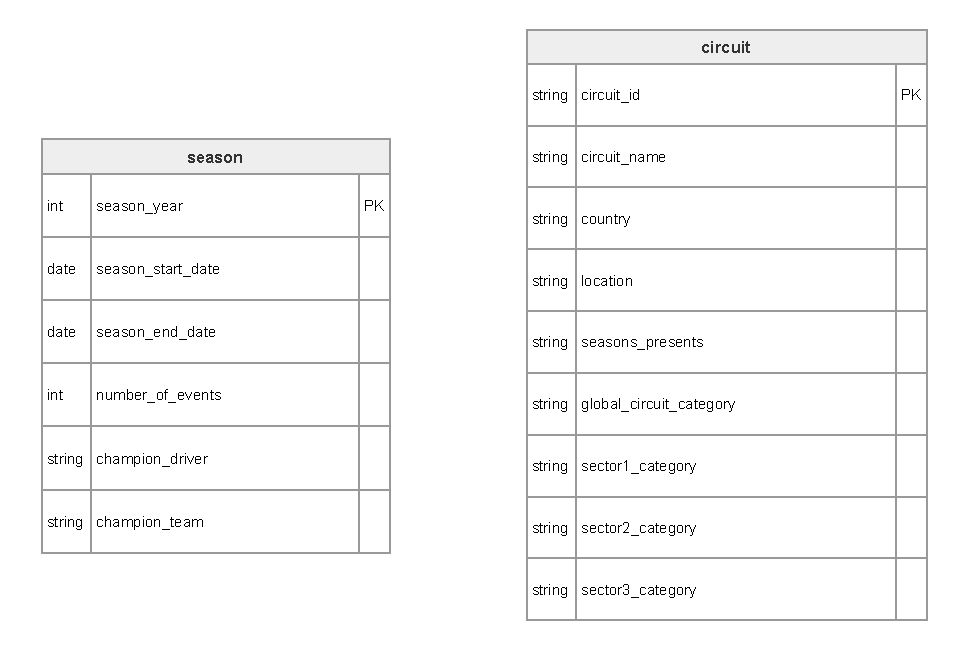
\includegraphics[width=0.90\textwidth]{image/domain_tables.pdf}
	\caption{Season and circuit domain tables introduced from documented external knowledge.}
	\end{figure}

	\newpage
	\subsection{Re-engineered Tables}
	
	The third visual representation shows the set of re-engineered tables after the transformation phase, but before the final conceptual and logical diagrams are presented.
	The goal is to show how the raw and domain tables are restructured into a coherent set of relations.
	
	\begin{figure}[H]
	\centering
	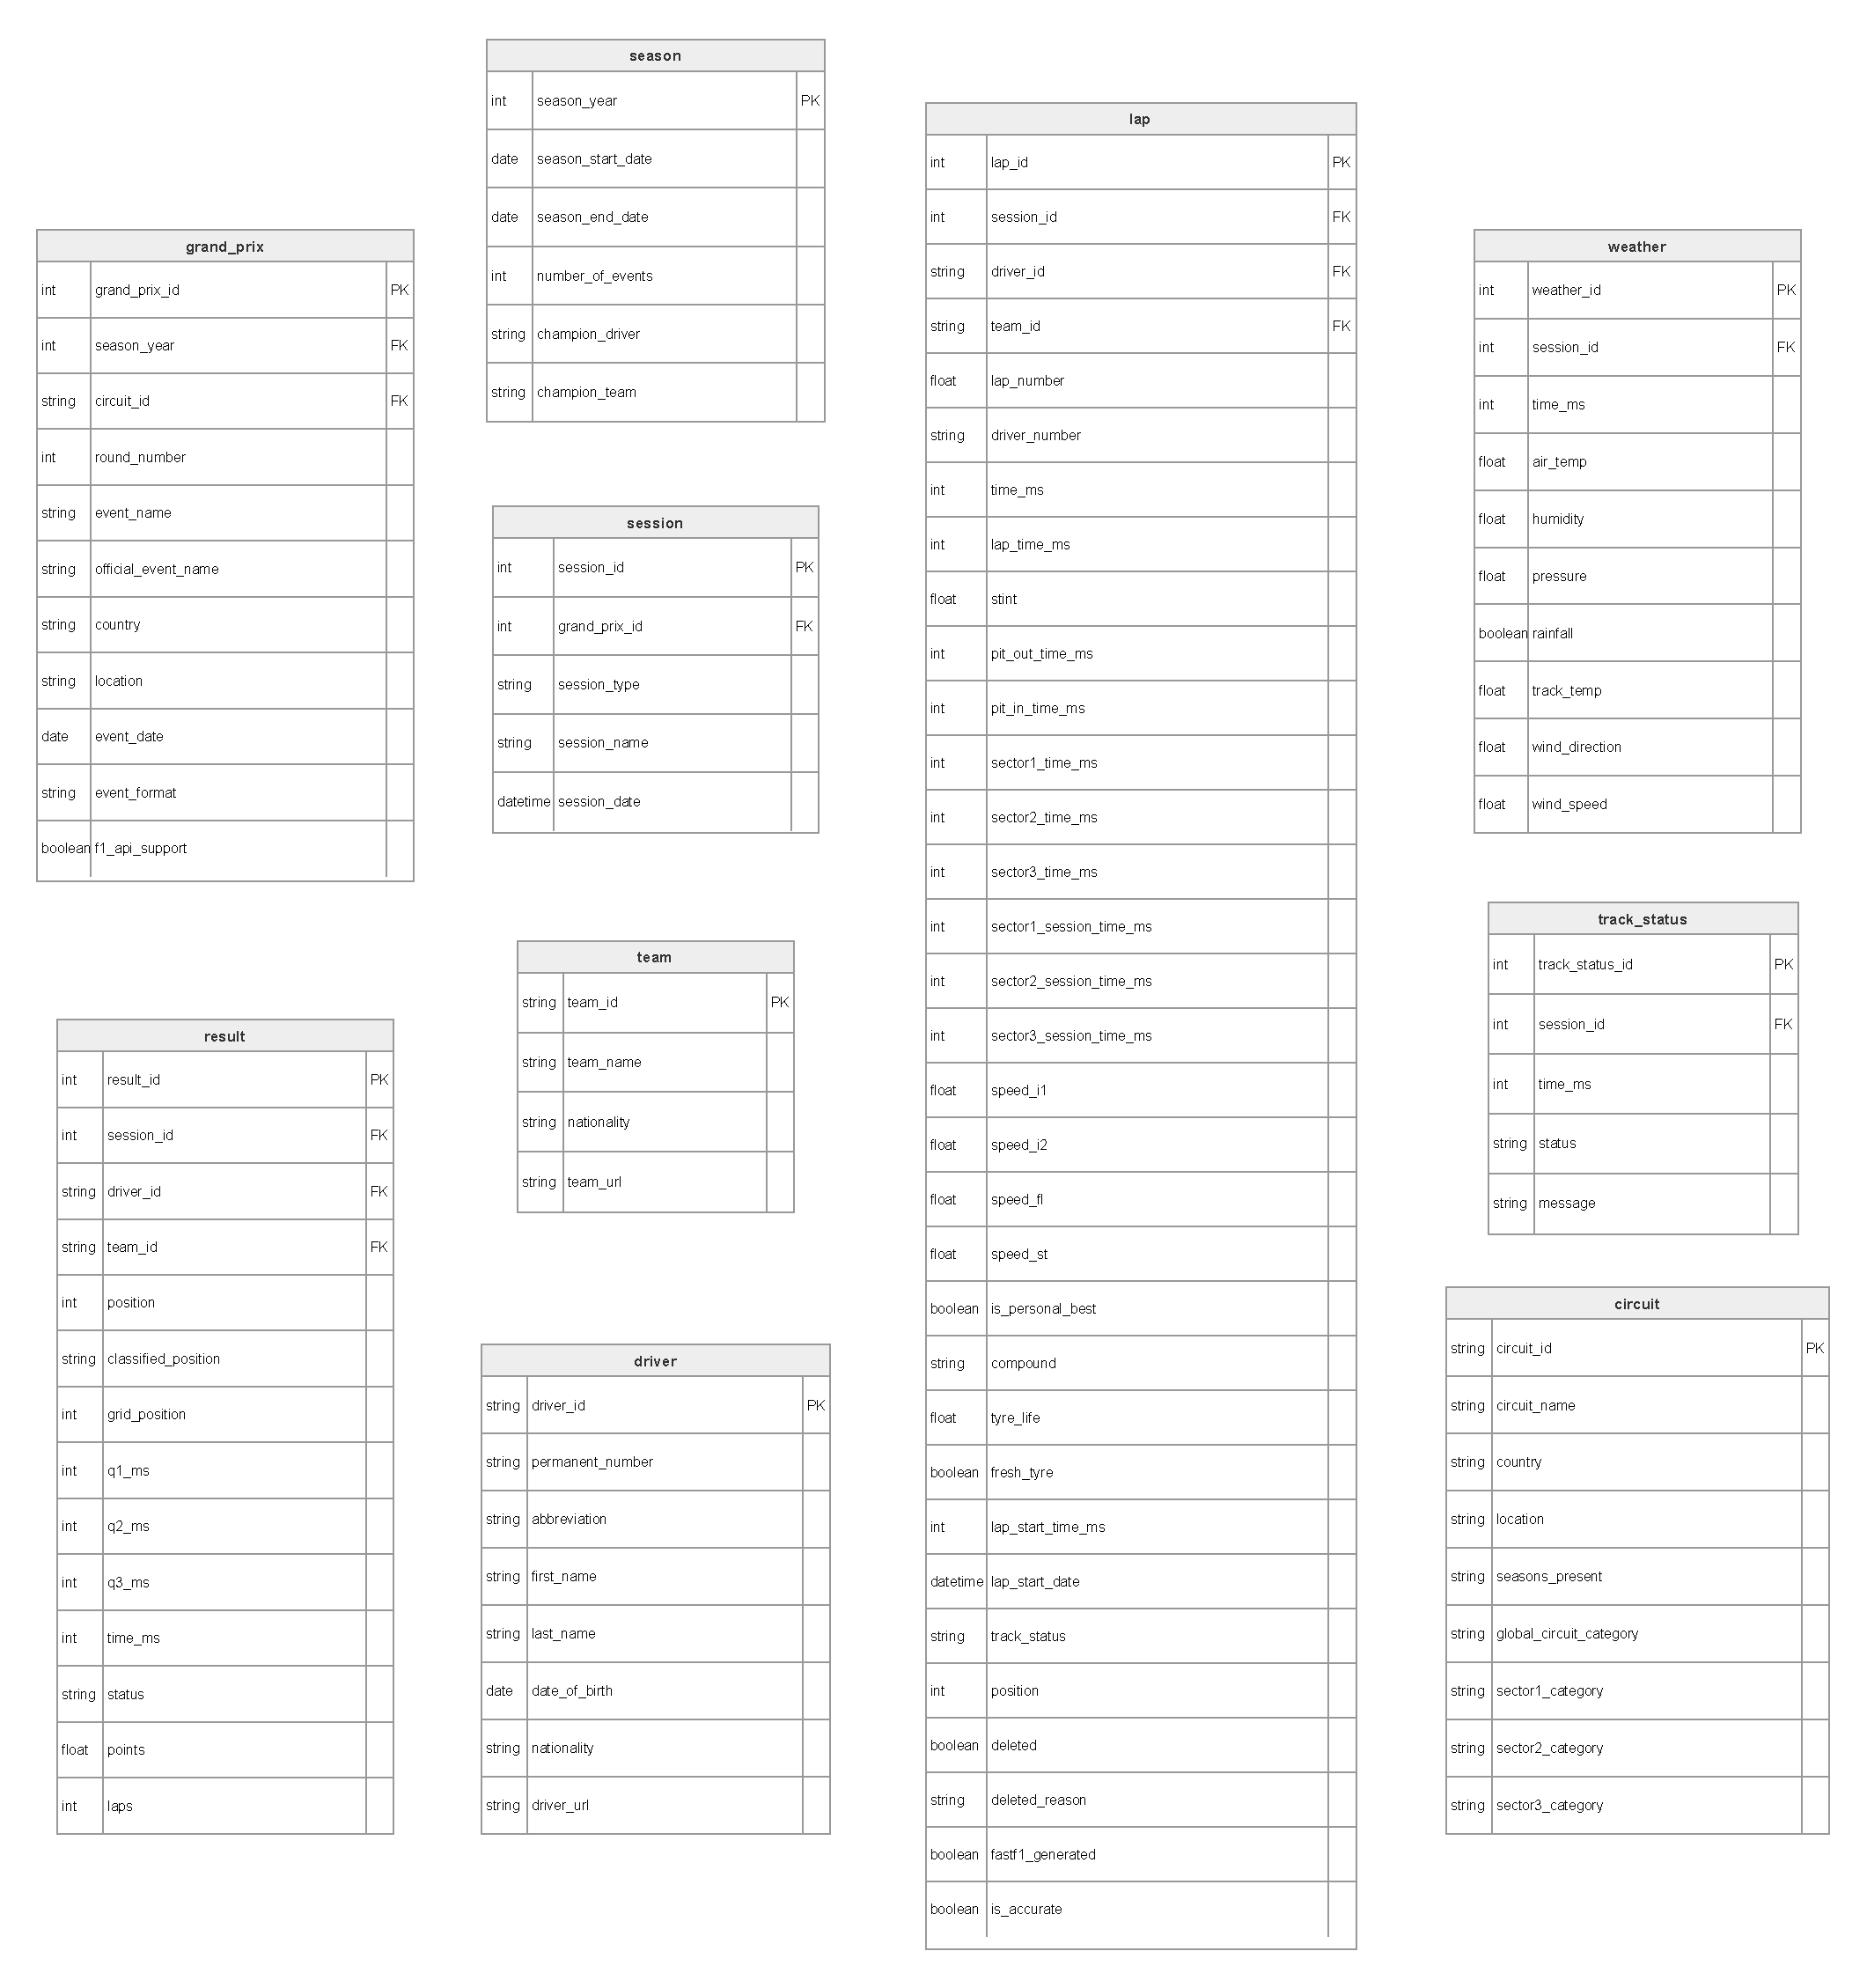
\includegraphics[width=1\textwidth]{image/re_engineer_tables.pdf}
	\caption{Tables produced by the re-engineering process before PostgreSQL loading.}
	\end{figure}
	
	\newpage
	\subsection{E/R Diagram}
	
	The fourth visual representation is the Entity--Relationship diagram of the reconciled database.
	At this level, the structure is represented conceptually, using entities and relationships.
	
	
	The E/R diagram uses a more user-friendly notation in order to make the
	main entities and relationships easier to understand at a conceptual level. Therefore, some
	attribute names may be shown in a simplified form, and not all implementation-level
	attributes are necessarily included in the diagram.
	
	The purpose of the E/R diagram is to describe the semantic structure of the domain and
	the main connections between entities. By contrast, the logical relational schema is the
	representation that is closer to the actual database implementation. The logical schema
	uses the real table names, real attribute names, primary keys, foreign keys, and naming
	conventions adopted in PostgreSQL.
	

	
	\begin{figure}[H]
	\centering
	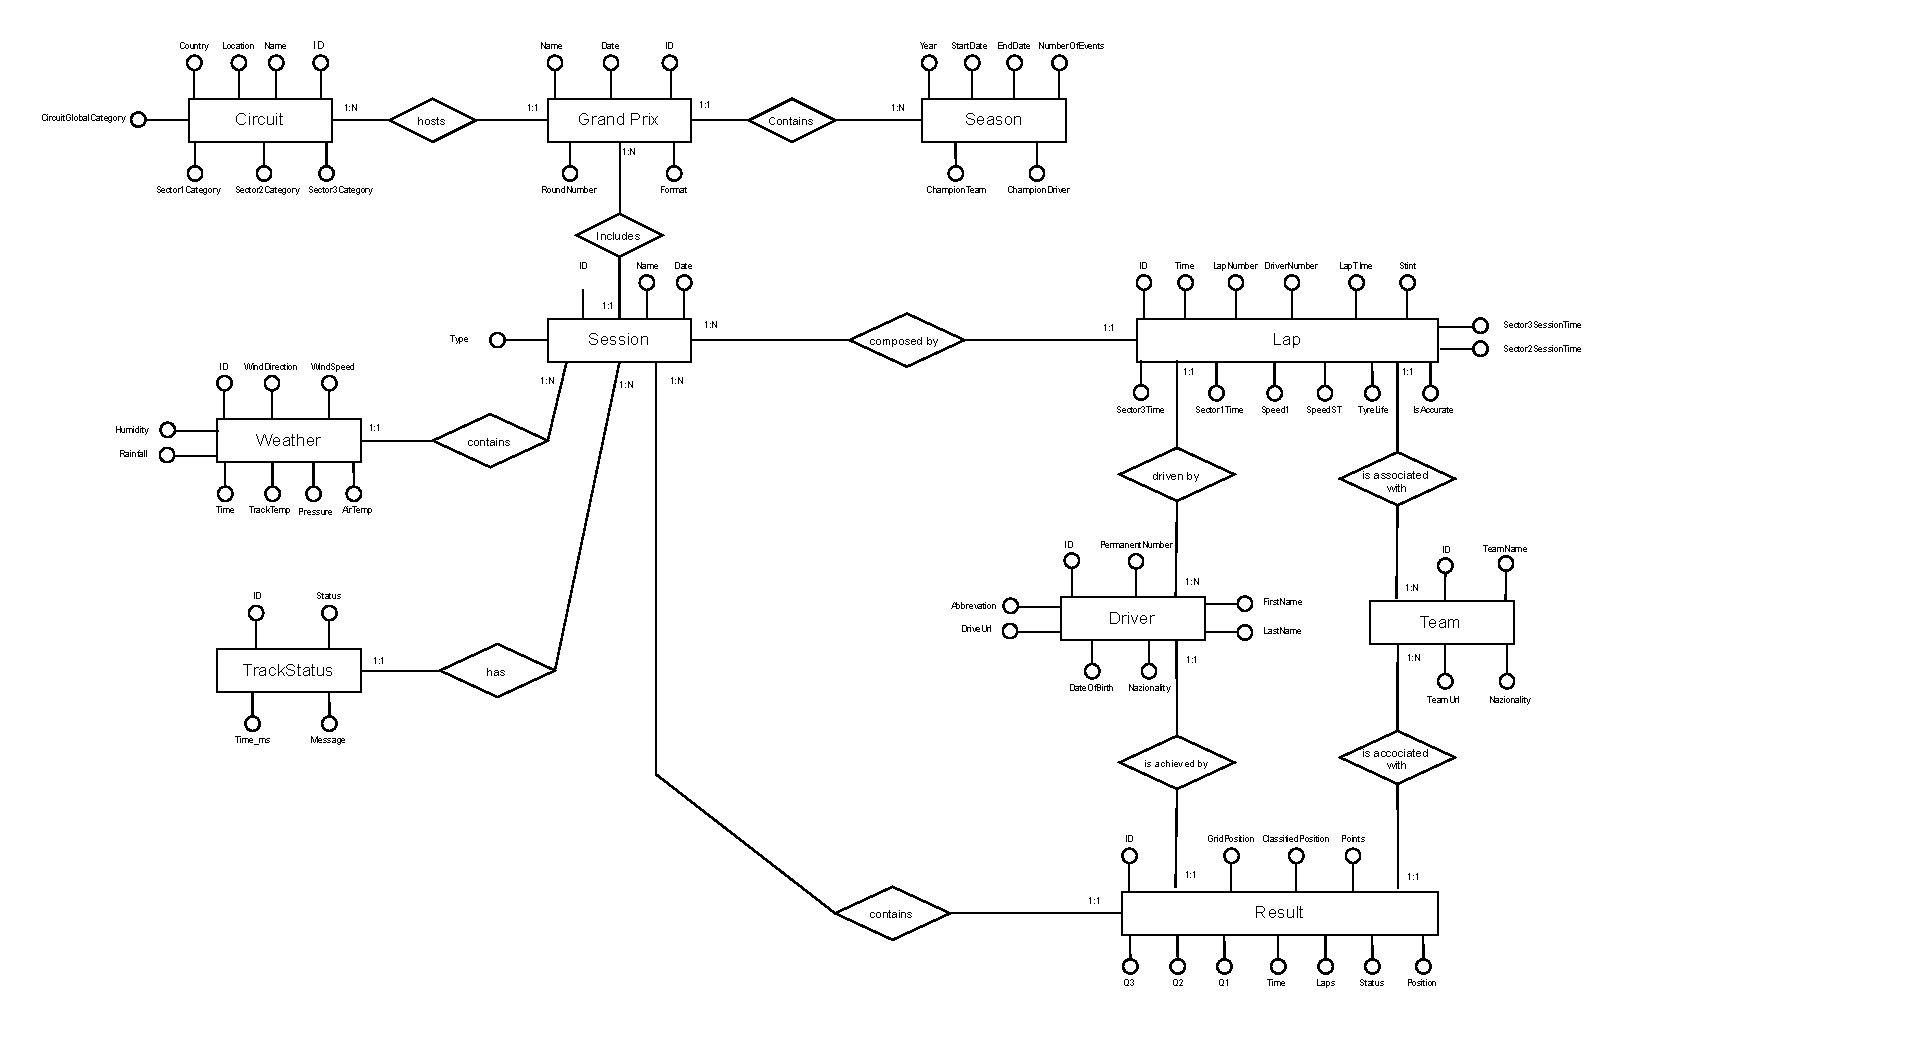
\includegraphics[width=1\textwidth]{image/e_r.pdf}
	\caption{Entity--Relationship schema of the normalized reconciled database.}
	\end{figure}
	
	\newpage
	\subsection{Logical Schema}
	
	The fifth visual representation is the logical relational schema derived from the E/R design.
	At this level, the implementation-oriented structure is shown explicitly, including associative tables, primary keys, and foreign keys.
	
	\begin{figure}[H]
	\centering
	
\includegraphics[width=0.90\textwidth]{image/logical_schema.pdf}
	\caption{Logical relational schema of the normalized reconciled database.}
	\end{figure}

	
	% =================================================
	\section{Conclusion}
	% =================================================
	
	This document has described the full re-engineering phase that transforms the raw data extracted from FastF1 and Ergast into a relational structure suitable for a reconciled PostgreSQL database.

	
	The final output of this phase is a coherent set of re-engineered CSV files ready to be loaded into PostgreSQL.



	The next document will address the subsequent stage of the project, namely the assessment of data quality and data cleaning tasks, followed by the conceptual design activities required for the future construction of the data warehouse.

\end{document}
